\documentclass{beamer}
\mode<presentation>
\usepackage{amsmath}
\usepackage{amssymb}
%\usepackage{advdate}
\usepackage{adjustbox}
\usepackage{subcaption}
\usepackage{enumitem}
\usepackage{multicol}
\usepackage{mathtools}
\usepackage{listings}
\usepackage{url}
\def\UrlBreaks{\do\/\do-}
\usetheme{Boadilla}
\usecolortheme{lily}
\setbeamertemplate{footline}
{
  \leavevmode%
  \hbox{%
  \begin{beamercolorbox}[wd=\paperwidth,ht=2.25ex,dp=1ex,right]{author in head/foot}%
    \insertframenumber{} / \inserttotalframenumber\hspace*{2ex} 
  \end{beamercolorbox}}%
  \vskip0pt%
}
\setbeamertemplate{navigation symbols}{}

\providecommand{\nCr}[2]{\,^{#1}C_{#2}} % nCr
\providecommand{\nPr}[2]{\,^{#1}P_{#2}} % nPr
\providecommand{\mbf}{\mathbf}
\providecommand{\pr}[1]{\ensuremath{\Pr\left(#1\right)}}
\providecommand{\qfunc}[1]{\ensuremath{Q\left(#1\right)}}
\providecommand{\sbrak}[1]{\ensuremath{{}\left[#1\right]}}
\providecommand{\lsbrak}[1]{\ensuremath{{}\left[#1\right.}}
\providecommand{\rsbrak}[1]{\ensuremath{{}\left.#1\right]}}
\providecommand{\brak}[1]{\ensuremath{\left(#1\right)}}
\providecommand{\lbrak}[1]{\ensuremath{\left(#1\right.}}
\providecommand{\rbrak}[1]{\ensuremath{\left.#1\right)}}
\providecommand{\cbrak}[1]{\ensuremath{\left\{#1\right\}}}
\providecommand{\lcbrak}[1]{\ensuremath{\left\{#1\right.}}
\providecommand{\rcbrak}[1]{\ensuremath{\left.#1\right\}}}
\theoremstyle{remark}
\newtheorem{rem}{Remark}
\newcommand{\sgn}{\mathop{\mathrm{sgn}}}
\providecommand{\abs}[1]{\left\vert#1\right\vert}
\providecommand{\res}[1]{\Res\displaylimits_{#1}} 
\providecommand{\norm}[1]{\lVert#1\rVert}
\providecommand{\mtx}[1]{\mathbf{#1}}
\providecommand{\mean}[1]{E\left[ #1 \right]}
\providecommand{\fourier}{\overset{\mathcal{F}}{ \rightleftharpoons}}
%\providecommand{\hilbert}{\overset{\mathcal{H}}{ \rightleftharpoons}}
\providecommand{\system}{\overset{\mathcal{H}}{ \longleftrightarrow}}
	%\newcommand{\solution}[2]{\textbf{Solution:}{#1}}
%\newcommand{\solution}{\noindent \textbf{Solution: }}
\providecommand{\dec}[2]{\ensuremath{\overset{#1}{\underset{#2}{\gtrless}}}}
\newcommand{\myvec}[1]{\ensuremath{\begin{pmatrix}#1\end{pmatrix}}}
\let\vec\mathbf

\lstset{
%language=C,
frame=single, 
breaklines=true,
columns=fullflexible
}

\numberwithin{equation}{section}

\title{MATGEO Presentation}
\author{Dhawal \\ ee24btech11015,\\IIT Hyderabad.}

\date{\today} 
\begin{document}

\begin{frame}
\titlepage
\end{frame}

\section*{Outline}
\begin{frame}
\tableofcontents
\end{frame}
\section{Problem}
\begin{frame}
\frametitle{Problem Statement}
%
 Find the area enclosed by the parabola $4y = 3x^2$ and the line $2y = 3x+12$. 
 \begin{table}[h!]    
  \centering
  
\begin{tabular}[12pt]{ |c| c| c|}
    \hline
    \textbf{Variable} & \textbf{Description} & \textbf{Values} \\ 
    \hline
    AB & Length & 6 cm \\
    \hline
    BC & Length & 8 cm \\
    \hline
    $\angle ABC$ & Angle & \ang{60}\\
    \hline 
    $\vec{A}$ & Point & $(6,0)$ \\
    \hline
    $\vec{B}$ & Origin & $(0,0)$ \\
    \hline
    $\vec{C}$ & To find & ? \\
    \hline
    \end{tabular}


  \caption{Variables given}
  \label{tab 1.4.9.2}
\end{table}


\end{frame}

%\subsection{Literature}
\section{Solution}
\subsection{Matrix Equation}
\begin{frame}
\frametitle{Matrix Equation}
%\framesubtitle{Literature}
Parabola P in terms of matrix:
\begin{align}
P=\text{g}\brak{\vec{x}}=\vec{x}^{\top}\vec{V}\vec{x}+2\vec{u}^{\top}\vec{x}+f=0
\end{align}
Where:
\begin{align}
\vec{V}=\myvec{3&&0\\0&&0} \hspace{1cm} \vec{u}=\myvec{0\\-2} \hspace{1cm} f=0
\end{align}
Line L
\begin{align}
	L: \quad \vec{x} = \vec{h} + \kappa \vec{m} \quad \kappa \in \mathbb{R}
\end{align}
Where:
\begin{align}
\vec{h}=\myvec{0\\6} \hspace{1cm} \vec{m}=\myvec{1\\\frac{3}{2}}
\end{align}

\end{frame}
\subsection{Point of Intersection}
\begin{frame}
\frametitle{Point of Intersection}
Point of intersection of line L and parabola P:
\begin{align}
	\vec{x}_i = \vec{h} + \kappa_i \vec{m}
\end{align}
Where:
\begin{align}
	\kappa_i = \frac{1}
{
\vec{m}^{\top}\vec{V}\vec{m}
}
\lbrak{-\vec{m}^{\top}\brak{\vec{V}\vec{h}+\vec{u}}}
\pm
\rbrak{\sqrt{
\sbrak{
\vec{m}^{\top}\brak{\vec{V}\vec{h}+\vec{u}}
}^2
	-\text{g}
\brak
{\vec{h}
}
\brak{\vec{m}^{\top}\vec{V}\vec{m}}
}
}
\end{align}
Finding $\text{g}\brak{\vec{h}}$:
\begin{align}
	\text{g}\brak{\vec{h}}=-24
\end{align}
Finding $\kappa_i$:
\begin{align}
	\kappa_i=4 \text{ and } -2
\end{align}
So Points of intersection are:
\begin{align}
 \vec{A}=\myvec{4\\12} , \vec{B}=\myvec{-2\\3}
\end{align}
\end{frame}
\subsection{Area}
\begin{frame}
\frametitle{Area}

Area between the curves:
\begin{align}
     \int_{-2}^{4}\abs{1.5x+6-0.75x^2}\,dx =27
\end{align}
So Area between the graphs is 27.\\



\end{frame}


\subsection{PLot}
\begin{frame}[fragile]
\frametitle{Plot}

\begin{figure}[h!]
   \centering
   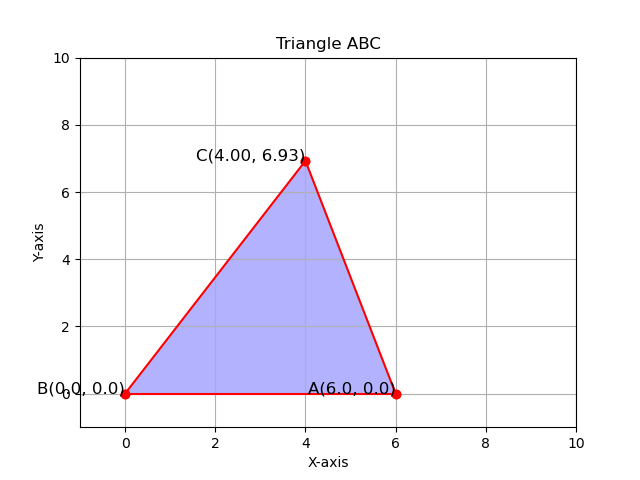
\includegraphics[width=0.9\linewidth]{Figure_1.png}
	\caption{Area Enclosed by parabola and line. }
   \label{stemplot}
\end{figure}
\end{frame}

\section{C Code}
\begin{frame}[fragile]
\frametitle{C Code for generating points on line}
\begin{lstlisting}[language=C]
#include <stdio.h>

void generate_line_points(double m, double c, double x_start, double x_end, double step, double *x_vals, double *y_vals, int *n) {
    int i = 0;
    for (double x = x_start; x <= x_end; x += step) {
        x_vals[i] = x;
        y_vals[i] = m * x + c;  // Equation: y = mx + c
        i++;
    }
    *n = i;  // Number of points generated
}
    \end{lstlisting}
\end{frame}
\begin{frame}[fragile]
\frametitle{C Code for generating points on parabola}
\begin{lstlisting}[language=C]
#include <stdio.h>
#include <stdlib.h>

// Function to generate points on the parabola y = a * x^2 + b * x + c
void generate_parabola_points(double a, double b, double c, double x_start, double x_end, double step, double* x_points, double* y_points) {
    int index = 0;
    for (double x = x_start; x <= x_end; x += step) {
        x_points[index] = x;
        y_points[index] = a * x * x + b * x + c;
        index++;
    }
}
}
\end{lstlisting}
\end{frame}


\section{Python Code}
\begin{frame}[fragile]
\frametitle{Python Code for Plotting}
\begin{lstlisting}[language=Python]
import numpy as np
import matplotlib.pyplot as plt
import ctypes
from scipy.optimize import fsolve
from scipy.integrate import quad

line_lib = ctypes.CDLL('./line_points.so')
parabola_lib = ctypes.CDLL('./parabola_points.so')

line_lib.generate_line_points.argtypes = [ctypes.c_double, ctypes.c_double, ctypes.c_double, ctypes.c_double, ctypes.c_double, ctypes.POINTER(ctypes.c_double), ctypes.POINTER(ctypes.c_double)]
parabola_lib.generate_parabola_points.argtypes = [ctypes.c_double, ctypes.c_double, ctypes.c_double, ctypes.c_double, ctypes.c_double, ctypes.c_double, ctypes.POINTER(ctypes.c_double), ctypes.POINTER(ctypes.c_double)]

\end{lstlisting}
\end{frame}

\begin{frame}[fragile]
\frametitle{Python Code for Plotting}
\begin{lstlisting}[language=Python]
n_points = 1000
x_points = np.linspace(-10, 10, n_points)
y_line_points = np.zeros(n_points, dtype=np.float64)
y_parabola_points = np.zeros(n_points, dtype=np.float64)

x_start, x_end = -10.0, 10.0
step = (x_end - x_start) / n_points

line_lib.generate_line_points(1.5, 6.0, x_start, x_end, step, x_points.ctypes.data_as(ctypes.POINTER(ctypes.c_double)), y_line_points.ctypes.data_as(ctypes.POINTER(ctypes.c_double)))
parabola_lib.generate_parabola_points(0.75, 0, 0, x_start, x_end, step, x_points.ctypes.data_as(ctypes.POINTER(ctypes.c_double)), y_parabola_points.ctypes.data_as(ctypes.POINTER(ctypes.c_double)))
def line_eq(x):
    return 1.5 * x + 6  # Line equation: y = 1.5x + 6

\end{lstlisting}
\end{frame}

\begin{frame}[fragile]
\frametitle{Python Code for Plotting}
\begin{lstlisting}[language=Python]
def parabola_eq(x):
    return 0.75 * x ** 2  # Parabola equation: y = 0.75x^2
def equations(x):
    return parabola_eq(x) - line_eq(x)

# Find the intersection points using fsolve
x_intersect_1 = fsolve(equations, -5)[0]  # First intersection, close to -5
x_intersect_2 = fsolve(equations, 5)[0]   # Second intersection, close to 5

y_intersect_1 = line_eq(x_intersect_1)  # y-coordinate of first intersection
y_intersect_2 = line_eq(x_intersect_2)  # y-coordinate of second intersection
def integrand(x):
    return abs(parabola_eq(x) - line_eq(x))
area, _ = quad(integrand, x_intersect_1, x_intersect_2)
print(f"Area between the line and the parabola: {area:.4f}")



\end{lstlisting}
\end{frame}

\begin{frame}[fragile]
\frametitle{Python Code for Plotting}
\begin{lstlisting}[language=Python]
plt.figure(figsize=(10, 6))
plt.plot(x_points, y_line_points, 'r', label='Line: y = 1.5x + 6')
plt.plot(x_points, y_parabola_points, 'g', label='Parabola: y = 0.75x^2')
plt.fill_between(x_points, y_line_points, y_parabola_points, 
                 where=((x_points >= x_intersect_1) & (x_points <= x_intersect_2)),
                 color='gray', alpha=0.5, label='Area between')
plt.scatter([x_intersect_1, x_intersect_2], [y_intersect_1, y_intersect_2], color='blue', s=100, zorder=5)
plt.text(x_intersect_1, y_intersect_1, f'({x_intersect_1:.2f}, {y_intersect_1:.2f})', fontsize=12, ha='right')
plt.text(x_intersect_2, y_intersect_2, f'({x_intersect_2:.2f}, {y_intersect_2:.2f})', fontsize=12, ha='left')
plt.legend()
plt.title('Area Between Line and Parabola')
plt.grid(True)
plt.show()

\end{lstlisting}
\end{frame}

\end{document}
